\documentclass{jhwhw}
\usepackage[utf8]{inputenc}
\usepackage{amsmath}
\usepackage{amssymb}
\usepackage{braket}
\usepackage{tikz}
\usepackage{forest}
\usepackage{booktabs}
\usepackage{color,soul}
\usepackage{enumitem}
\usepackage{adjustbox}
\usepackage[spanish]{babel}
\newcommand{\subscript}[2]{$#1 _ #2$}
\renewcommand{\thesection}{\arabic{section}}
\renewcommand{\thesubsection}{\arabic{subsection}}
\newcommand{\mytitle}{Act 4.1 Practicando las maquinas de Turing}
\usepackage{graphicx}

\begin{document}

\author{Juan Pablo Salazar-A01740200}
\title{\mytitle}

\maketitle

\subsection{$a(a|b)*b$}
\begin{center}
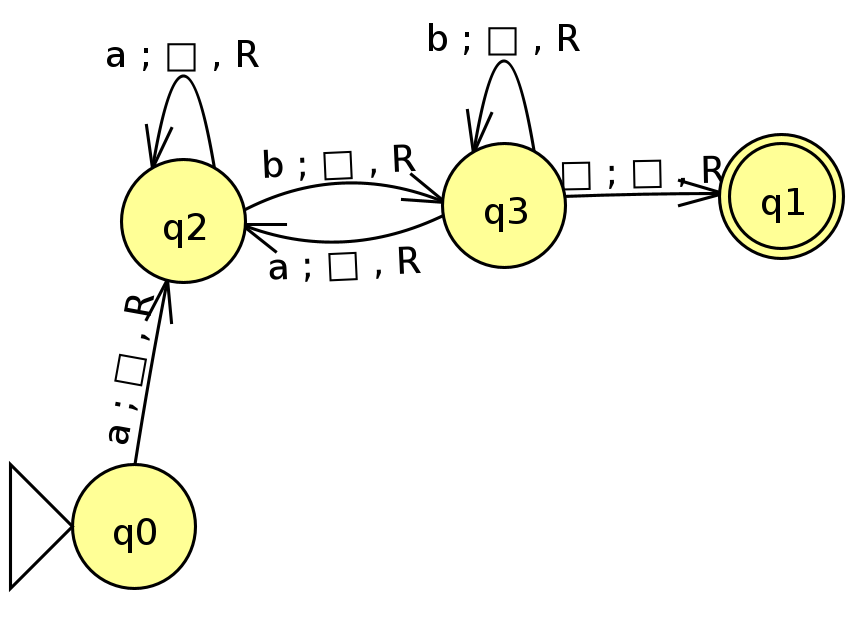
\includegraphics[width=0.5\linewidth]{imgs/maquina1.png}
\begin{table}[h]
\begin{tabular}{l|l}
$Q$      & $\{q0,q1,q2,q3\}$\\
$\Sigma$ &  {a,b}\\
$\Gamma$ &  $\{\square , a,b\}$\\
$\delta$  &  $\{(q0,a,(q2,\square,R)),(q2,a,(q2,\square,R)),...\}$\\
$q$      & q0 \\
$a$      & q1 \\
$r$      & {q0,q2,q3}
\end{tabular}
\end{table}
\end{center}

\subsection{$<(/|\varepsilon)(o|u)l>$}
\begin{center}
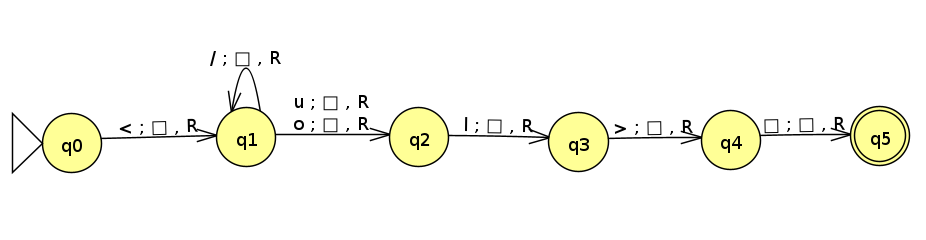
\includegraphics[width=\linewidth]{imgs/maquina2.png}
\begin{table}[h]
\begin{tabular}{l|l}
$Q$      & $\{q0,q1,q2,q3,q4,q5\}$\\
$\Sigma$ &  $\{<,/,o,u,l,>\}$\\
$\Gamma$ &  $\{\<,/,o,u,l,>,\square\}$\\
$\delta$  &  $\{(q0,<,(q1,\square,R)),(q1,/,(q1,\square,R)),...\}$\\
$q$      & q0 \\
$a$      & q5 \\
$r$      & $\{q0,q1,q2,q3,q4\}$
\end{tabular}
\end{table}
\end{center}

\subsection{$\{a^nb^n:n\ge0\}$}
\begin{center}
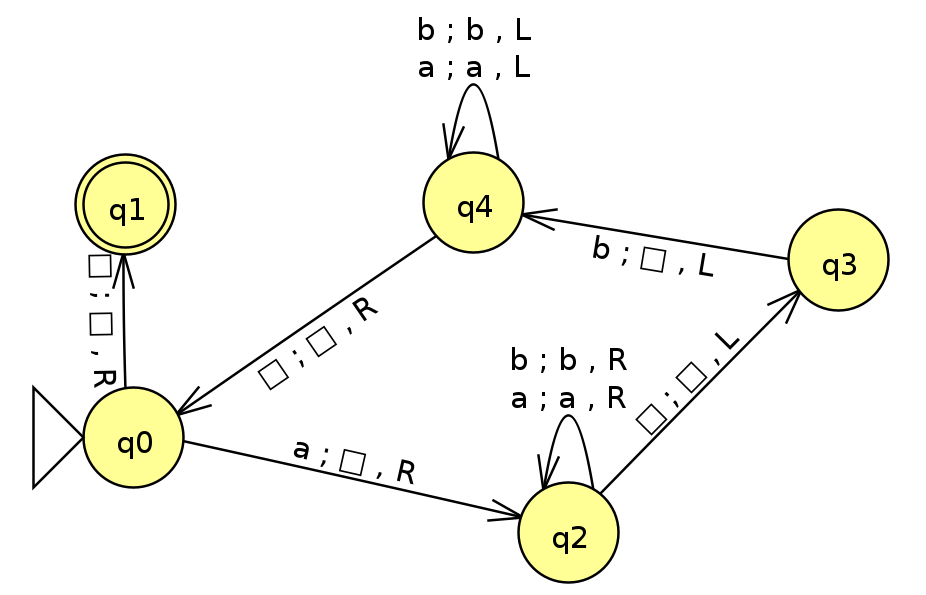
\includegraphics[width=\linewidth]{imgs/maquina3.png}
\begin{table}[h]
\begin{tabular}{l|l}
$Q$      & $\{q0,q1,q2,q3,q4\}$\\
$\Sigma$ &  $\{a,b\}$\\
$\Gamma$ &  $\{a,b,\square\}$\\
$\delta$  &  $\{(q0,\square,(q1,\square,R)),(q0,a,(q2,\square,R)),...\}$\\
$q$      & q0 \\
$a$      & q1 \\
$r$      & $\{q0,q2,q3,q4\}$
\end{tabular}
\end{table}
\end{center}

\subsection{$\{w|a \in w, b\in w, \#a = \#b\}$}
\begin{center}
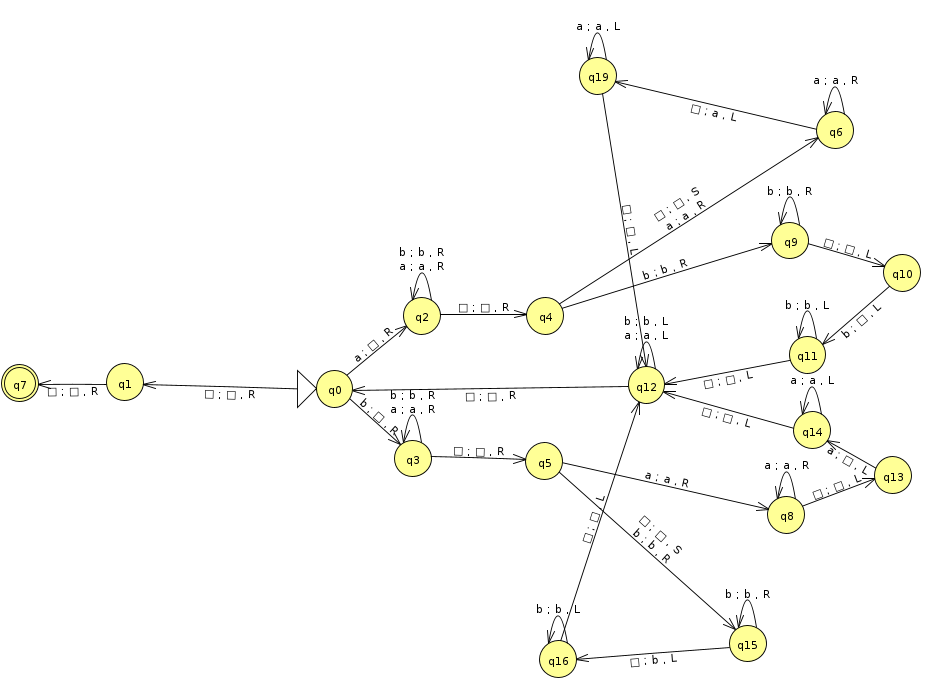
\includegraphics[width=\linewidth]{imgs/maquina4.png}
\begin{table}[h]
\begin{tabular}{l|l}
$Q$      & $\{q0,q1,q2,q3,...,q19\}$\\
$\Sigma$ &  $\{a,b\}$\\
$\Gamma$ &  $\{a,b,\empty\}$\\
$\delta$  &  $\{(q0,\square,(q1,\square,R)),(q0,b,(q3,\square,R)),...\}$\\
$q$      &  q0\\
$a$      &  q7\\
$r$      & $\{q0,q1,q2,q3,q4,q5,q6,q8,...,q19\}$
\end{tabular}
\end{table}
\end{center}

\end{document}